
% Inbuilt themes in beamer
\documentclass{beamer}
\renewcommand{\tablename}{Tabla}

% Theme choice:
% \usetheme{CambridgeUS}
\usetheme{Darmstadt}
\usepackage{svg}
\usepackage{amsmath}

% DECIR: Introducir la tesis:
% Buenos días, gracias a todos por estar aquí, mi nombre es Luis Ernesto.
% Hoy se presenta la defensa de la tesis NOMBRE DE TESIS.
\title{Extracción automática de argumentos en textos de opinión en la prensa cubana} 
\author{Luis Ernesto Ibarra Vázquez}
\institute{Universidad de La Habana}
\date{13 de diciembre del 2022}
\logo{
\includegraphics[keepaspectratio=true,height=2cm,width=2cm]{Graphics/uhlogo.pdf}}


\begin{document}

% Title page frame
\begin{frame}
    \titlepage 
\end{frame}

% Remove logo from the next slides
\logo{}

\section{Introducción}
\begin{frame}{Argumentación}
    \begin{block}{Argumentación}
        Es una actividad verbal, social y racional destinada a convencer
        a un crítico razonable de la aceptabilidad de un punto de vista mediante la presentación 
        de una constelación de proposiciones que justifican o refutan la proposición
        expresada en el punto de vista.
    \end{block}
    % DECIR: Ejemplos de argumentación:
    % - Persona explicando una situación y cómo esta le afecta
    % - En discursos políticos en las que se desea convencer a las personas que se afilien al partido
    \pause
    \begin{block}{Importancia}
        \begin{itemize}
            \pause
            \item Obtener puntos de vista en los textos, obteniendo información sobre 
            los argumentos principales utilizados.
            \pause
            \item Detectar sobre qué se basan las justificación de 
            afirmaciones. 
        \end{itemize}
    \end{block}
\end{frame}

\begin{frame}{Extracción de argumentos}
    % DECIR: Para el estudio computacional de la argumentación se forma
    \begin{block}{Extracción de Argumentos}
        \pause 
        Es la rama del Procesamiento de Lenguaje Natural encargada del
        estudio de métodos para la extracción automática de las \textbf{estructuras argumentativas}
        de los textos y su posterior procesamiento.
    \end{block}
    \pause 
    % DECIR: Las estructuras argumentativas (Notar el bold) son las 
    % partes estructurales de la argumentación en los textos.
    % Estas se componen por:
    \begin{block}{Estructuras Argumentativas}
        \begin{itemize}
            \pause
            \item Unidades de discurso argumentativas (UDA).
            % DECIR: Definición de UDA:
            % Un segmento de texto que juega un solo rol para el argumento analizado, 
            % y es delimitado por segmentos vecinos que tienen roles diferentes o ningún rol
            \pause
            \item Relaciones entre las UDAs.
        \end{itemize}
    \end{block}
\end{frame}

\begin{frame}[t]{Tareas de la extracción de argumentos}
    % DECIR: Dadas las definiciones anteriores se conciben 4 tareas
    % necesarias para la extracción de las estructuras argumentativas de
    % texto.
    % NOTA: A medida que se vaya haciendo progreso en el slide, ir mencionando
    % lo que ocurre, el marcado de UDAs, su clasificación y explicar la parte de las 
    % relaciones, que no se entiende a la primera seguro
    % NOTA: Leer el ejemplo para dar contexto hablado de este.
    \begin{block}{Tareas de extracción de argumentos}
        \begin{enumerate}
            \item<2-> Extracción de las UDAs.
            \item<5-> Clasificación de las UDAs.
            \item<8-> Extracción de las relaciones entre las UDAs.
            \item<10-> Clasificación de las relaciones entre las UDAs.
        \end{enumerate}
    \end{block}

    En primer lugar, \only<3->{[}\textbf<3->{el correo electrónico puede contar como uno de los resultados
    más beneficiosos de la tecnología moderna}\only<3->{]}\begin{onlyenv}<6->{$_{\mathrm{Afirmaci\acute{o}n}}$}\end{onlyenv}. 
    \only<4->{[}\textbf<4->{Años atrás, las personas pagaban gran cantidad de dinero para 
    enviar sus cartas y sus pagos estaban sujetos al peso de sus cartas o paquetes y muchos accidentes 
    podrían causar problemas que causarían que el correo no fuera enviado}\only<4->{]}\begin{onlyenv}<7->{$_{\mathrm{Premisa}}$}\end{onlyenv}\begin{onlyenv}<9->{$, _{-1}$}\end{onlyenv}\begin{onlyenv}<11->{$, _{\mathrm{apoyo}}$}\end{onlyenv}.

    % DECIR: Como se puede observar la representación directamente sobre el texto no es la mejor, 
    % sobre todo en la parte de visualizar las relaciones. Para esto una vía alternativa de modelar 
    % el problema consiste en hacerlo mediante un grafo.

\end{frame}

\begin{frame}{Estructuras argumentativas como grafo}
    \only<1>{Extracción de las UDAs:}
    \only<2>{Clasificación de las UDAs:}
    \only<3>{Extracción de las relaciones entre las UDAs:}
    \only<4>{Clasificación de las relaciones entre las UDAs:}
    \vspace{0.5cm}
    \begin{onlyenv}<1>
        \begin{columns}
            \begin{column}{0.32\textwidth}
                
            \end{column}
            \begin{column}{0.68\textwidth}
                \includesvg[scale=.6]{Graphics/Estructuras_argumentativas1.svg}
            \end{column}
        \end{columns}
    \end{onlyenv}
    \begin{onlyenv}<2>
        \begin{figure}
            \includesvg[scale=.6]{Graphics/Estructuras_argumentativas2.svg}
        \end{figure}
    \end{onlyenv}
    \begin{onlyenv}<3>
        \begin{figure}
            \includesvg[scale=.6]{Graphics/Estructuras_argumentativas3.svg}
        \end{figure}
    \end{onlyenv}
    \begin{onlyenv}<4>
        \begin{figure}
            \includesvg[scale=.6]{Graphics/Estructuras_argumentativas.svg}
        \end{figure}
    \end{onlyenv}

\end{frame}

\section{Propuesta}

\begin{frame}{Objetivos y propuesta}
    % DECIR: Con lo anterior, el objetivo de este trabajo consiste en:
    \begin{block}{Objetivo}
        \pause
        Proponer un algoritmo para la extracción y
        análisis de estructuras argumentativas en textos de la prensa cubana.
    \end{block}
    \pause  
    % DECIR: Para esto se propone la creación de 
    \begin{block}{Propuesta}
        \pause
        \begin{itemize}
            \item Dos modelos de aprendizaje profundo para:
            \begin{enumerate}
                \pause
                \item Extracción y clasificación de UDAs.
                \pause
                \item Extracción y clasificación de relaciones.
            \end{enumerate}
            % DECIR: En la extracción de argumentos no se presentan 
            % conjuntos de datos en español para el entrenamiento de dichos modelos 
            % por lo tanto se necesita conseguir estos a partir de los presentes en otros lenguajes.
            % Para resolver esto se propone:
            \pause
            \item Proyección de conjuntos de datos al español para el entrenamiento de los modelos
            propuestos. 
        \end{itemize}
    \end{block}
\end{frame}

\begin{frame}{Modelación del problema de segmentación y clasificación de UDAs}
    % DECIR: Se modela como un problema de clasificación de secuencia a secuencia en el que a cada 
    % elemento de la secuencia de entrada (SLIDE) se le asocia una etiqueta BIOES (SLIDE y explicar BIOES).
    % NOTA: Delimitar la UDA.
    % A esta etiqueta BIOES se le asocia otra clasificación (SLIDE) que 
    % codifica la clasificación del tipo de UDA.
    \begin{columns}
        \begin{column}{0.6\textwidth}
            \begin{itemize}
                \item<3-> B: Inicio de segmento.
                \item<4-> I: Dentro del segmento.
                \item<5-> E: Final del segmento.
                \item<6-> S: Segmento de un elemento.
                \item<7-> O: Afuera del segmento.
            \end{itemize}
        \end{column}
        \begin{column}{0.2\textwidth}<2->
            En\\
            primer\\
            lugar\\
            ,\\
            el\\
            correo\\
            electrónico\\
            \dots\\
            de\\
            la\\
            tecnología\\
            moderna\\
            .
        \end{column}
        \begin{column}{0.2\textwidth}<8->
            O\\
            O\\
            O\\
            O\\
            B\only{-Afirmación}<9->\\
            I\only{-Afirmación}<9->\\
            I\only{-Afirmación}<9->\\
            \dots\\
            I\only{-Afirmación}<9->\\
            I\only{-Afirmación}<9->\\
            I\only{-Afirmación}<9->\\
            E\only{-Afirmación}<9->\\
            O
        \end{column}
        
    \end{columns}
\end{frame}

\begin{frame}{Segmentación y clasificación de UDAs}
    % DECIR: La entrada del algoritmo consiste en texto (SLIDE),
    % este es procesado (SLIDE) al realizarle los procesos de tokenización y 
    % de anotación de partes de la oración. Con esta información se crea una 
    % secuencia de tokens representando a cada token con un embeddings que contiene
    % información semántica (GloVe), sintáctica (POS) y morfológica (Char info) con el 
    % objetivo de capturar la mayor cantidad de información del texto como los rasgos lingüísticos
    % que denotan a un texto como argumentativo.

    % DECIR: Esta secuencia de embedding es procesada por el modelo propuesto y (SLIDE)
    % la salida de este es arreglada la estructura BIOES, obteniendo finalmente las UDAs 
    % clasificadas.
    \begin{columns}
        \begin{column}{0.10\textwidth}
            \begin{block}{}
                Texto
            \end{block}
        \end{column}
        \begin{column}<2->{0.01\textwidth}
            \begin{math}
                \Rightarrow
            \end{math}
        \end{column}
        \begin{column}<3->{0.30\textwidth}
            \begin{block}{}
                Segmentación y clasificación de UDAs.
            \end{block}
        \end{column}
        \begin{column}<4->{0.01\textwidth}
            \begin{math}
                \Rightarrow
            \end{math}
        \end{column}
        \begin{column}<5->{0.25\textwidth}
            \includesvg[scale=0.3]{Graphics/UDAs.svg}
        \end{column}
    \end{columns}

    \vspace{1cm}

    \begin{columns}[T]
        \begin{column}<2->{0.5\textwidth}
            Procesamiento de entrada:
            \begin{itemize}
                \item Tokenización.
                \item Anotación de las partes de la oración.
                \item \textit{Embeddings}.
            \end{itemize}
        \end{column}
        \begin{column}<4->{0.5\textwidth}
            Procesamiento de salida:
            \begin{itemize}
                \item Arreglar el formato BIOES de las secuencias.
                \item Asignar una sola clasificación a cada segmento.
            \end{itemize}
        \end{column}
    \end{columns}
\end{frame}

\begin{frame}{Modelo de segmentación y clasificación de UDAs}
    % NOTA: Hacer referencia a los embeddings y a su concatenación 
    \begin{onlyenv}<1>
        \begin{center}
            \includesvg[scale=0.4]{Graphics/Modelo_segmenter_uda1.svg}
        \end{center}
    \end{onlyenv}
    % NOTA: Hacer referencia al procesamiento de la secuencia de embeddigns
    % - LSTM bidireccional
    % - Conexion residual
    % - Capa Densa
    % - CRF: Devuelve la secuencia de mayor probabilidad dado los features 
    \begin{onlyenv}<2>
        \begin{center}
            \includesvg[scale=0.4]{Graphics/Modelo_segmenter_uda2.svg}
        \end{center}
    \end{onlyenv}
\end{frame}

\begin{frame}{Modelación del problema de extracción y clasificación de realciones}
    % DECIR: El problema se modela como uno de clasificación en el que, dado dos UDAs,
    % se clasifica la relación entre estas. Para completar el grafo del documento (SLIDE),
    % se tiene un conjunto de UDAs en él, por cada 
    % par (SLIDE) de UDAs válidas se realiza la predicción de la relación (SIDE).
    % Conformando el resultado final.

    \begin{columns}
        \pause
        \begin{column}{0.3\textwidth}
            \begin{itemize}
                \item UDA1 
                \item UDA2 
                \item UDA3
            \end{itemize}
        \end{column}
        \pause
        \begin{column}{0.4\textwidth}
            \begin{itemize}
                \item (UDA1, UDA2)
                \item (UDA1, UDA3)
                \item (UDA2, UDA1)
                \item (UDA2, UDA3)
                \item (UDA3, UDA1)
                \item (UDA3, UDA2)
            \end{itemize}
        \end{column}
        \pause
        \begin{column}{0.4\textwidth}
            \begin{itemize}
                \item No Relacionado
                \item No Relacionado
                \item Apoyo 
                \item No Relacionado
                \item Ataque
                \item Ataque
            \end{itemize}
        \end{column}
    \end{columns}

\end{frame}

\begin{frame}{Extracción y clasificación de relaciones}

    \begin{columns}
        \begin{column}{0.25\textwidth}
            \includesvg[scale=0.2]{Graphics/UDAs.svg}
        \end{column}
        \begin{column}<2->{0.01\textwidth}
            \begin{math}
                \Rightarrow
            \end{math}
        \end{column}
        \begin{column}<3->{0.30\textwidth}
            \begin{block}{}
                Extracción y clasificación de las relaciones.
            \end{block}
        \end{column}
        \begin{column}<4->{0.01\textwidth}
            \begin{math}
                \Rightarrow
            \end{math}
        \end{column}
        \begin{column}<5->{0.25\textwidth}
            \includesvg[scale=0.2]{Graphics/UDAs_relacionadas.svg}
        \end{column}
    \end{columns}

    \vspace{1cm}

    \begin{columns}[T]
        \begin{column}<2->{0.5\textwidth}
            Procesamiento de entrada:
            \begin{itemize}
                \item Creación de tuplas conteniendo la UDA fuente y la UDA objetivo y distancia argumentativa.
                \item Tokenización.
                \item \textit{Embeddings}.
            \end{itemize}
        \end{column}
        \begin{column}<4->{0.5\textwidth}
            Procesamiento de salida:
            \begin{itemize}
                \item Asignar etiqueta a la relación en dependencia del resultado.
            \end{itemize}
        \end{column}
    \end{columns}
\end{frame}

\begin{frame}{Modelo de extracción y clasificación de relaciones}
    \begin{onlyenv}<1-2>
        \begin{columns}
            \begin{column}<1->{0.5\textwidth}
                \begin{center}
                    \includesvg[scale=0.4]{Graphics/Modelo_link_prediction_1.svg}
                \end{center}
            \end{column}
            \begin{column}<2->{0.5\textwidth}
                \begin{center}
                    \includesvg[scale=0.4]{Graphics/Modelo_link_prediction_2.svg}
                \end{center}
            \end{column}
        \end{columns}
    \end{onlyenv}
    \begin{onlyenv}<3>
        \begin{center}
            \includesvg[scale=0.40]{Graphics/Modelo_link_prediction_3.svg}
        \end{center}
    \end{onlyenv}
\end{frame}

\section{Experimentación}

% DECIR: Dada la falta de un corpus en el dominio de las cartas a la dirección se
% entrenó el modelo propuesto con diferentes conjuntos de datos.
% El modelo aprende el criterio de segmentación y clasificación de las UDAs y de las
% relaciones directamente del conjunto de datos.
% NOTA: Destacar el desbalance, escasez y heterogeniedad de los datos
\begin{frame}[t]{Conjuntos de datos}
    \textbf{Conjuntos de datos:}
    \begin{itemize}
        \item Cartas a la Dirección.
        \item<2-> Ensayos Argumentativos.
        \item<3-> Cornell eRulemaking Corpus (CDCP).
        \item<4-> Abstracts Randomized Control Trials (AbsTRCT).
    \end{itemize}
    \vspace{0.5cm}
    \uncover<2->{\textbf{Caractecrísticas:}}
    \begin{itemize}
        \item<2-> Documentos: \only<2>{286 textos argumentativos escritos por estudiantes sobre temáticas diferentes}\only<3>{731 comentarios escritos por usuarios en un sitio web}\only<4>{500 resúmenes sobre investigaciones de enfermedades}.
        \item<2-> Segmentado por: \only<2>{Cláusula}\only<3>{Oración}\only<4>{Oración}.
        \item<2-> Clasificación de UDAs: \only<2>{\textit{Major claim} (12\%), \textit{claim} (25\%) y \textit{premise} (63\%)}\only<3>{\textit{Policy} (17\%), \textit{value} (45\%), \textit{fact} (16\%), \textit{testimony} (21\%) y \textit{reference} (1\%)}\only<4>{\textit{Major claim} (3\%), \textit{claim} (30\%) y \textit{premise} (67\%)}.
        \item<2-> Clasificación de relaciones: \only<2>{\textit{Attack} (6\%) y \textit{support} (94\%)}\only<3>{\textit{Reason} (97\%) y \textit{evidence} (3\%)}\only<4>{\textit{Support} (85\%), \textit{partial-attack} (12\%) y \textit{attack} (3\%)}.
    \end{itemize}
\end{frame}

\begin{frame}{Selección del modelo}
    % DECIR: Para la selección del modelo se establecieron diferentes variantes y estas fueron entrenadas 
    % en el conjunto de datos de Ensayos Persuasivos. Se selecciona el mejor modelo de acuerdo a un 
    % criterio y finalmente los mejores hiperparámetros son utilizados en el entrenamiento de los 
    % demás conjuntos de datos. Las métricas utilizadas como criterio son:

    \pause
    \begin{block}{Métricas}
        \begin{itemize}
            % DECIR: Se utiliza en la clasificación multimodal y se define como el promedio de 
            % F1 de las clases presentes.
            \pause
            \item Macro F1.
            % DECIR: Se define como la proporcion de aciertos del modelo 
            \pause
            \item \emph{Accuracy}.
            % DECIR: Es una medida específica de la segmentación, en la que el número
            % representa el porciento del segmento que tiene que coincidir para 
            % que se considere válido el emparejamiento.
            \pause
            \item 100\%F1 y 50\%F1.
        \end{itemize}
    \end{block}

    \pause
    Todas estas medidas oscilan entre 0 y 1 donde 1 es el mejor resultado posible.

\end{frame}

\begin{frame}{Selección del modelo de segmentación}
    \begin{onlyenv}<1>
        \begin{table}
            \begin{center}
                \begin{tabular}{|l|c|c|c|c|c|c|} \hline
                Modelos 		& POS       & Char-CNN  & Char-LSTM & Res       & Norm      & Densa  \\ \hline
                Modelo 1		& $\times$	& $\times$    & $\times$    & $\times$	& $\times$    & $\times$ \\ \hline
                Modelo 2		& $\times$	& $\checkmark$    & $\checkmark$    & $\checkmark$	& $\checkmark$    & $\times$ \\ \hline
                Modelo 3		& $\checkmark$	& $\checkmark$    & $\checkmark$    & $\checkmark$	& $\checkmark$    & $\times$ \\ \hline
                Modelo 4		& $\checkmark$	& $\checkmark$    & $\checkmark$    & $\checkmark$	& $\checkmark$    & $\checkmark$ \\ \hline
                \end{tabular}
            \caption{Variantes de arquitectura de los modelos de segmentación de UDA.}
            \end{center}
        \end{table}
    \end{onlyenv}
    \begin{onlyenv}<2>
        \begin{figure}
            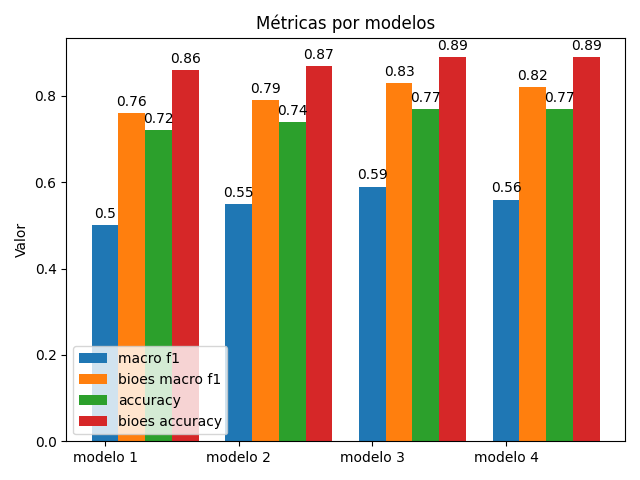
\includegraphics[scale=0.6]{Graphics/persuasive_essays_all_linked_macro_micro_metrics.png}
            \caption{Métricas de ensayos persuasivos en la clasificación de etiquetas.}
        \end{figure}
    \end{onlyenv}
    \begin{onlyenv}<3>
        \begin{figure}
            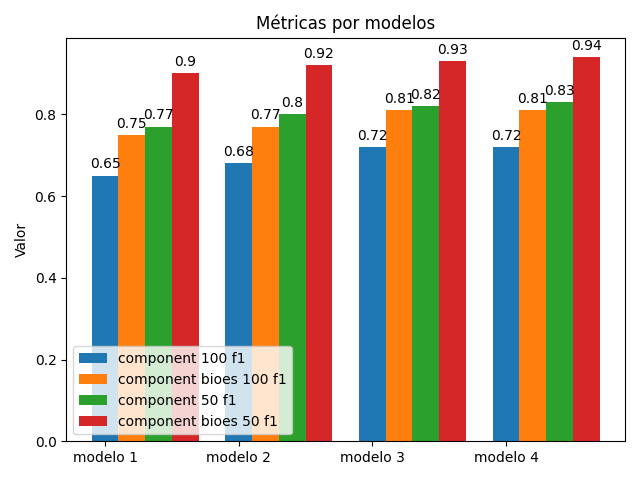
\includegraphics[scale=0.6]{Graphics/persuasive_essays_all_linked_components.png}
            \caption{Métricas de ensayos persuasivos en la segmentación de UDAs.}
        \end{figure}
    \end{onlyenv}
    % DECIR: Por los resultados obtenidos se seleccionan los valores del modelo 4 para el 
    % entrenamiento del modelo en los demás conjuntos de datos
    \begin{onlyenv}<4>
        \begin{table}
            \begin{center}
                \begin{tabular}{|l|c|c|c|c|c|c|} \hline
                Modelos 		& POS       & Char-CNN  & Char-LSTM & Res       & Norm      & Densa  \\ \hline
                Modelo 1		& $\times$	& $\times$    & $\times$    & $\times$	& $\times$    & $\times$ \\ \hline
                Modelo 2		& $\times$	& $\checkmark$    & $\checkmark$    & $\checkmark$	& $\checkmark$    & $\times$ \\ \hline
                Modelo 3		& $\checkmark$	& $\checkmark$    & $\checkmark$    & $\checkmark$	& $\checkmark$    & $\times$ \\ \hline
                \textbf{Modelo 4}		& $\checkmark$	& $\checkmark$    & $\checkmark$    & $\checkmark$	& $\checkmark$    & $\checkmark$ \\ \hline
                \end{tabular}
            \caption{Variantes de arquitectura de los modelos de segmentación de UDA.}
            \end{center}
        \end{table}
    \end{onlyenv}
    \begin{onlyenv}<5->
        \begin{table}
            \begin{center}
                \scalebox{0.85}{
                \begin{tabular}{|l|c|c|c|c|} \hline
                Corpus		            & Macro F1	        & \emph{Accuracy}     & 100\%F1       & 50\%F1  	     \\ \hline
                Ensayos Argumentativos  & 0,56 / 0,82		& 0,77 / 0,89	      & 0,72 / 0,81   & 0,83 / 0,94      \\ \hline
                CDCP		            & 0,45 / 0,56		& 0,66 / 0,96	      & 0,61 / 0,82   & 0,68 / 0,93      \\ \hline
                AbsTRCT	                & 0,50 / 0,79		& 0,87 / 0,91	      & 0,61 / 0,66   & 0,75 / 0,82      \\ \hline
                \end{tabular}
                }
            \caption{Métricas del segmentador en su versión completa y BIOES.}\label{table:test_metrics_segmenter}
            \end{center}
        \end{table}
    \end{onlyenv}
\end{frame}

\begin{frame}{Selección del modelo de predicción de enlace}
    \begin{onlyenv}<2>
        \begin{table}
            \begin{center}
                \scalebox{0.7}{
                \begin{tabular}{|l|c|c|c|c|c|c|} \hline
                Modelos   	             & Atención      & Pooling  & \emph{Dropout}   & T. de aprendizaje & Paciencia & Devolver mejores     \\ \hline
                Modelo 1            	 & $\times$	     &  5       & 0,5              & 0,0015            & 10	       & $\checkmark$        \\ \hline
                Modelo 2                 & $\times$	 	 & 10       & 0,1              & 0,003             & 5	       & $\times$            \\ \hline
                Modelo 3	             & $\checkmark$	 &  1       & 0,1              & 0,003             & 5	       & $\times$            \\ \hline
                Modelo 4	             & $\checkmark$	 &  1       & 0,5              & 0,0015            & 10	       & $\checkmark$        \\ \hline
                \end{tabular}
                }
            \caption{Variantes de arquitectura de los modelos de predicción de enlaces.}
            \end{center}
        \end{table}
    \end{onlyenv}
    \begin{onlyenv}<3>
        \begin{figure}
            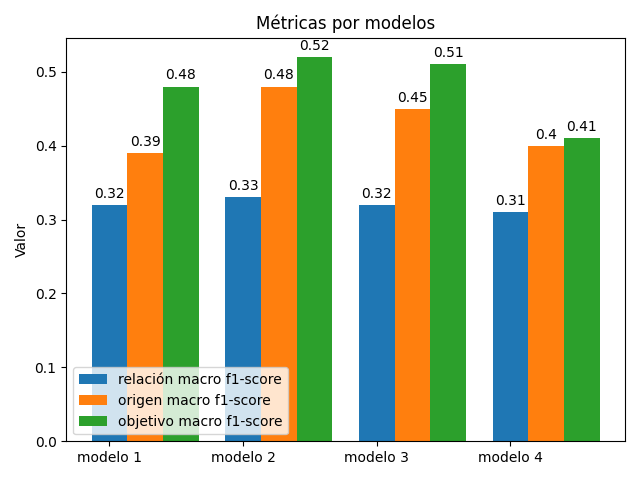
\includegraphics[scale=0.6]{Graphics/persuasive_essays_all_linked_all_relation_f1_scores.png}
            \caption{Métricas de ensayos persuasivos en la clasificación de enlaces y UDAs.}
        \end{figure}
    \end{onlyenv}
    \begin{onlyenv}<4>
        \begin{figure}
            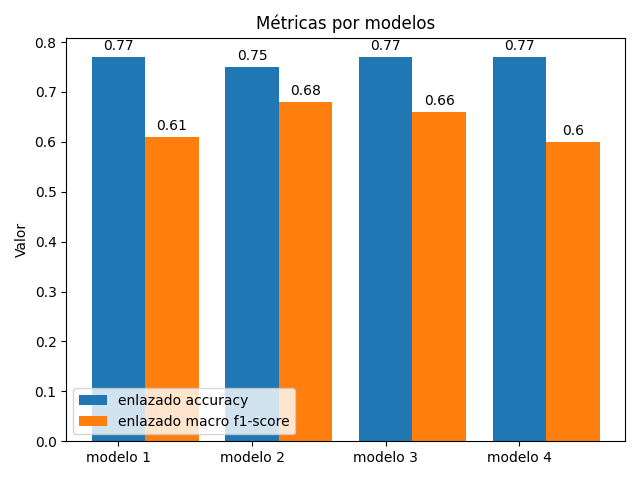
\includegraphics[scale=0.6]{Graphics/persuasive_essays_all_linked_all_relation_linked.png}
            \caption{Métricas de ensayos persuasivos en la extracción de enlaces de UDAs.}
        \end{figure}
    \end{onlyenv}
    % DECIR: Por los resultados obtenidos se seleccionan los valores del modelo 2 para el 
    % entrenamiento del modelo en los demás conjuntos de datos
    \begin{onlyenv}<5>
        \begin{table}
            \begin{center}
                \scalebox{0.7}{
                \begin{tabular}{|l|c|c|c|c|c|c|} \hline
                Modelos   	             & Atención      & Pooling  & \emph{Dropout}   & T. de aprendizaje & Paciencia & Devolver mejores     \\ \hline
                Modelo 1            	 & $\times$	     &  5       & 0,5              & 0,0015            & 10	       & $\checkmark$        \\ \hline
                \textbf{Modelo 2}                 & $\times$	 	 & 10       & 0,1              & 0,003             & 5	       & $\times$            \\ \hline
                Modelo 3	             & $\checkmark$	 &  1       & 0,1              & 0,003             & 5	       & $\times$            \\ \hline
                Modelo 4	             & $\checkmark$	 &  1       & 0,5              & 0,0015            & 10	       & $\checkmark$        \\ \hline
                \end{tabular}
                }
            \caption{Variantes de arquitectura de los modelos de predicción de enlaces.}
            \end{center}
        \end{table}
    \end{onlyenv}
    \begin{onlyenv}<6->
        \begin{table}
            \begin{center}
                \scalebox{0.7}{
                \begin{tabular}{|l|c|c|c|c|} \hline
                Corpus		            & Macro F1 Clasif. & \emph{Acc.} Clasif. & Macro F1 Enlace & \emph{Acc.} Enlace \\ \hline
                Ensayos Argumentativos  & 0,33	   & 0,57            & 0,68	    		& 0,75	  \\ \hline
                CDCP		            & 0,37	   & 0,63	         & 0,79	    		& 0,68	  \\ \hline
                AbsTRCT	                & 0,39	   & 0,61	         & 0,83	    		& 0,74	  \\ \hline
                \end{tabular}
                }
            \caption{Métricas de predicción de relaciones de las pruebas del predictor de enlace.}\label{table:test_relation_metrics_link_predictor}
            \end{center}
        \end{table}
    \end{onlyenv}
\end{frame}

\begin{frame}[t]{Experimentación}
    Se anotaron las Cartas a la Dirección del periódico Granma con los modelos entrenados en los diferentes conjuntos de datos 
    para determinar el modelo que se ajusta a los datos, llegando a las siguientes consideraciones luego de
    analizar un subconjunto 15 pares de cartas seleccionadas:
    
    \begin{itemize}
        \begin{onlyenv}<2-5>
            \item AbsTRCT:
            \begin{itemize}
                \item<3-> Todas las UDAs son clasificadas como Premisa.
                \item<4-> Existen pocas relaciones extraídas.
                \item<5-> La precisión de las relaciones de \textit{partial-attack} es baja.
            \end{itemize}
        \end{onlyenv}
        \begin{onlyenv}<6-10>
            \item Ensayos Persuasivos:
            \begin{itemize}
                \item<7-> Mejora en cuanto a la variedad de las clasificaciones de las UDAs.
                \item<8-> Posee problemas de segmentación en la que la UDA se queda incompleta.
                \item<9-> Posee una gran cantidad de falsos positivos en las relaciones.
                \item<10-> No se encuentran relaciones de \textit{attack} anotadas.
            \end{itemize}
        \end{onlyenv}
        \begin{onlyenv}<11->
            \item CDCP:
            \begin{itemize}
                \item<12-> Mejora en la segmentación 
                (Las oraciones tienden a formar mejores UDAs en este tipo de texto).
                \item<13-> Disminuye la cantidad de falsos positivos en las relaciones.
                \item<14-> No posee una relación de ataque entre sus candidatos.
            \end{itemize}
        \end{onlyenv}
    \end{itemize}
    \only<15>{Se selecciona este conjunto de datos para la anotación final de las Cartas a la Dirección}
\end{frame}

\section{Conclusiones}

% DECIR: 
% - Streamlit: Tiene el objetivo de una interacción fácil con el software, permitiendo realizar todas 
% las actividades en sus versiones elementales. Inferencia de archivos, entrenamiento de modelo, 
% proyección de corpus.
% - Colab: Esta aplicacion tiene como principal objetivo el entrenamiento y exportación de los modelos.
% Aunque permite también realizar inferencia y visualización de resultados básica.
% - Brat: Este software permite la visualización de las estructuras argumentativas, además de poder
% editar estas.
\begin{frame}{Resultados}
    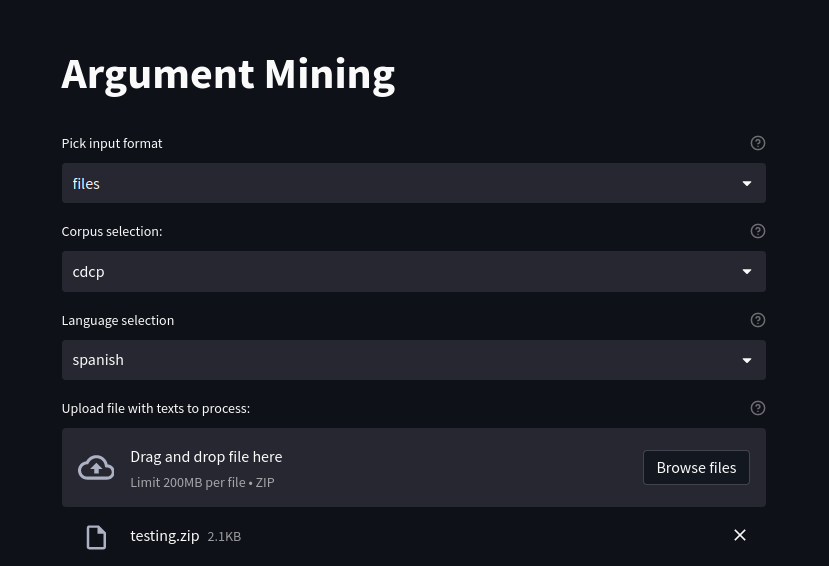
\includegraphics[keepaspectratio=true,height=\textheight,width=\textwidth]{Graphics/streamlit_app.png}<1>
    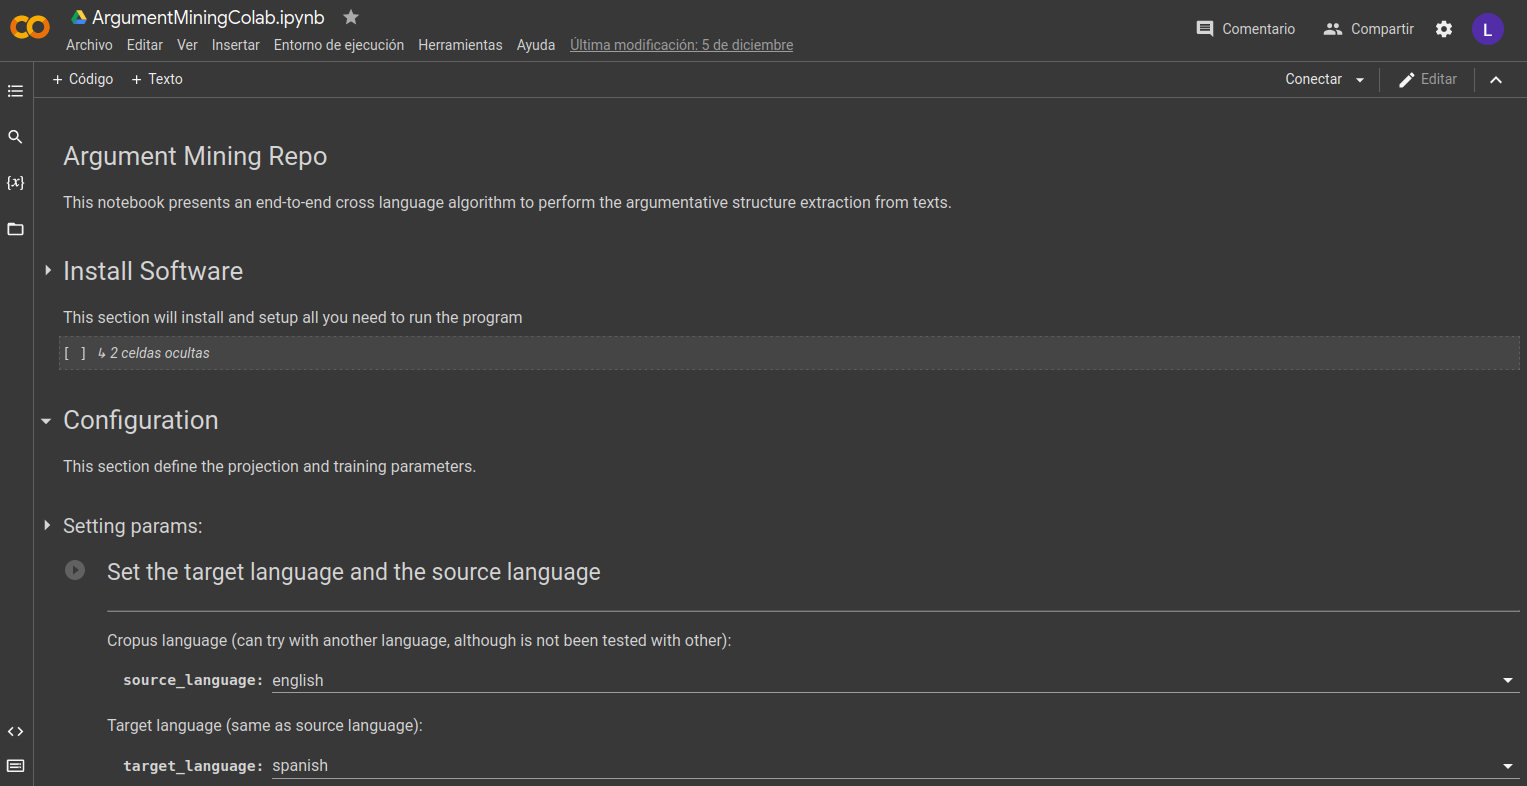
\includegraphics[keepaspectratio=true,height=\textheight,width=\textwidth]{Graphics/colab.png}<2>
    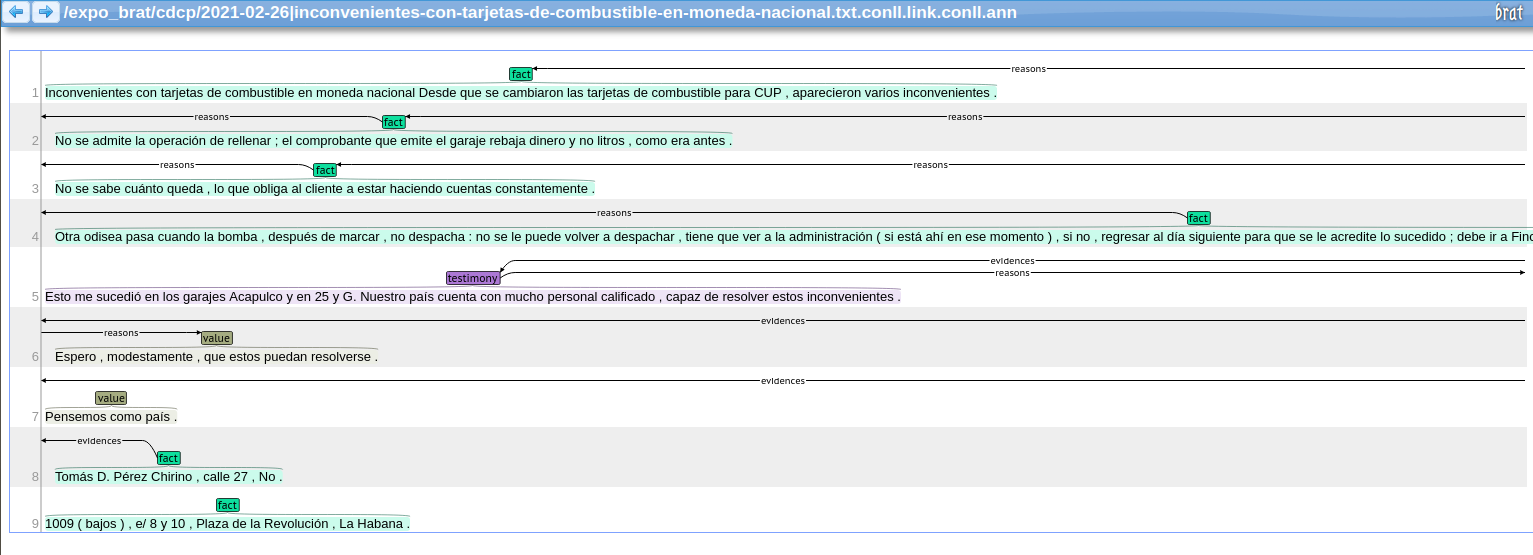
\includegraphics[keepaspectratio=true,height=\textheight,width=\textwidth]{Graphics/brat_cdcp_example.png}<3>
\end{frame}

\begin{frame}{Conclusiones}
    \begin{itemize}
        \item Se crean conjuntos de datos en español a partir de sus originales en inglés mediante la proyección de estos.
        \pause
        \item Se obtiene un conjunto de datos de Cartas a la Dirección.
        \pause
        \item Se presenta un software para la extracción y visualización de estructuras argumentativas.
        \pause
        \item Se etiquetan las estructuras argumentativas en las Cartas a la Dirección.
    \end{itemize}
\end{frame}

\begin{frame}{Recomendaciones}
    \begin{itemize}
        \item<1-> Supervisar la anotación de las Cartas a la Dirección con las estructuras argumentativas por lingüístas.
        \item<2-> Aplicar el uso de otros \textit{embeddings}, como BERT, entrenados sobre el conjunto 
        de datos extraído.
        \item<3-> Proponer un modelo capaz de tomar en cuenta el contexto del texto completo para la
        predicción y clasificación de enlaces, por ejemplo \textit{Graph Neural Networks}.
    \end{itemize}    
\end{frame}

% Title page frame
\logo{
\includegraphics[keepaspectratio=true,height=2cm,width=2cm]{Graphics/uhlogo.pdf}}
\begin{frame}
    \titlepage 
\end{frame}
\logo{}

\begin{frame}[t]{Preguntas del oponente}
    1. En el trabajo se utiliza GloVe y se menciona a BERT cómo una recomendación para mejorar la 
    solución. ¿Qué impidió el uso de BERT en primera instancia?

    % 1- No se usa BERT debido principalmente a un tema de tiempo, en los papers hablaban de
    % GloVe y otros embeddings en donde GloVe había obtenido buenos resultados, por eso se empezó
    % utilizando este embedding, luego apareció Bert y me pareció interesante probar su uso en el
    % modelo, ya que esta representación está dejando buenos resultados en las tareas de NLP. 
    
    % TODO Buscar articulos donde aparezca GloVe y Bert

    % Aunque la inclusión de BERT no es tarea complicada, los cambios a realizar en el modelo son mínimos
    % ya que solamente hace falta cambiar la capa de Embedding del modelo por la capa BERT devolviendo 
    % la representación vectorial correspondiente. Entre los modelos BERT existentes que pudiesen ser
    % utilizados se encuentran BETO https://github.com/dccuchile/beto y también en TensorFlow Hub
    % https://tfhub.dev/s?language=es&module-type=text-embedding&q=Bert
    % se encuentran cuatro modelos BERT, aunque estos son para el caso multi lenguaje (xlm_roberta_multi_cased).

    \begin{onlyenv}<2>
        \begin{figure}
            \includesvg[scale=0.4]{Graphics/Modelo_segmenter_uda1.svg}
        \end{figure}
    \end{onlyenv}
    \begin{onlyenv}<3>
        \begin{figure}
            \includesvg[scale=0.4]{Graphics/Modelo_segmenter_uda1_bert.svg}
        \end{figure}
    \end{onlyenv}
\end{frame}

\begin{frame}[t]{Preguntas del oponente}
    2. El paso del postprocesamiento de segmentación utiliza una serie de heurísticas. 
    ¿Puede proponer una idea de solución a este paso que utilice un enfoque de aprendizaje automático?

    % 2- Una propuesta podría ser que dado una ventana de procesamiento inválida devuelva una versión 
    % válida de esta. Se plantearía como un problema de clasificación entre las posibles ventanas válidas, 
    % manteniendo la ventana en un tamaño pequeño. El conjunto de datos se crearía con los mismos errores
    % que comente actualmente el modelo con respecto a sus etiquetas originales. Este modelo aún podría 
    % cometer errores en la inferencia debido a algún caso que no se vio u otra situación, por lo que igual 
    % se recomienda usar el algoritmo de heurística como fase final. 

    % El algoritmo utilizado para la corrección de las etiquetas corresponde de dos pasos. En primer 
    % lugar corregir la estructura BIOES de la secuencia y en segundo lugar corregir las metaetiquetas 
    % de las secuencias. En la primera sección el algoritmo utilizado consiste en mantener una ventana de 
    % tamaño 3 sobre la secuencia BIOES. Sobre dicha ventana se itera y al encontrarse una ventana BIOES
    % inválida se procede a arreglarla. Al analizar la ventana se asume que se desea arreglar la etiqueta 
    % del medio de esta teniendo como premisa que la primera etiqueta esta correctamente posicionada, a esta
    % primera etiqueta se le puede llamar como contexto de la ventana. Para arreglar se conciben dos casos:
    
    % Se tiene una ventana inválida y se tiene dos ventanas inválidas consecutivas. En el primer caso se hace 
    % el arreglo de la ventana de manera prefijada de acuerdo a para que la ventana sea válida. En el caso 
    % de que sean dos consecutivas se puede probar que solamente arreglando una de las dos ventanas se
    % devuelve una secuencia que no es necesaria hacerle cambios en estos dos lugares para que sea válida.
    % Para seleccionar cual segmento se arregla se crea una función de relevancia de error, la cual es escrita
    % a mano. 


    \begin{columns}[T]
        \begin{column}{0.3\textwidth}
            \pause
            Caso correcto:\\
            (O, O, B)\\
            \pause
            (O, B, I)\\
            \pause
        \end{column}
        \begin{column}{0.3\textwidth}
            Caso incorrecto:\\
            \pause
            (B, I, O)\\ 
            \pause
        \end{column}
        \begin{column}{0.3\textwidth}
            Casos posibles:\\
            \pause
            (B, E, O)\\
            (B, I, I)\\
            (B, I, E)\\
            % DECIR La ambiguedad presente en arreglar el segmento y como 
            % partiendo de las premisas anteriores se elimina o disminuye dicha ambiguedad
            % Solo es arreglar I que en este caso consiste en una sola forma. Solamente existe ambiguiedad
            % en los casos [E, S, O] _ [B, O, S] => [E, S, O] [S,O] [B, O, S], pero dado el dominio la opcion
            % de O es mejor
        \end{column}
    \end{columns}

    % Propuesta 1:

    % Dado una entrada de una ventana de tamaño 3 inválida de etiquetas BIOES, predecir cual es la secuencia
    % que arregla dicha ventana que minimiza la cantidad de errores comentidos en el proceso de inferencia.
    % El conjunto de datos se puede crear a partir de las etiquetas inferidas por el modelo y las etiquetas
    % reales presentes en los datos. El problema se puede modelar como uno de clasificación en el cual se 
    % las categorías son ventanas válidas BIOES. Aunque este procedimiento sigue estando propenso a errores.

    % Propuesa 2:

    % Dado que el arreglo de la ventana con las restricciones de arreglar solamente la etiqueta central 
    % no presenta ambigüedad, el problema recide
    % en encontrar la función que diga cual de las dos ventanas es la mejor a arreglar, donde mejor sea la que
    % minimice el error con las etiquetas reales. Esta variante no presentaría errores ya que el algoritmo
    % es el mismo.

\end{frame}

\begin{frame}[t]{Preguntas del oponente}
    3. ¿Cómo fue realizado el ajuste de hiperparámetros de los modelos propuestos durante la 
    experimentación? ¿Tiene alguna recomendación sobre ese proceso para futuras investigaciones?

    % 3- Un método de optimización de hiperparametros como grid search u otro no fue utilizado, el espacio 
    % de búsqueda de ellos es muy grande en comparación con el tiempo que se toma en entrenar el modelo. 
    % Como hiperparametros bases se eligieron los que proponían las investigaciones originales de los modelos 
    % los cuales ya presentaban un proceso de ajuste y sobre estos se eligieron variantes en cuanto a 
    % arquitecturas y features nuevos agregados (para ver 
    % cómo afectaba estos a los resultados) y se realizó en el caso del modelo de segmentación de modelos 
    % una pequeña búsqueda sobre el Learning rate, tamaño del pooling, dropout, entre otros.

    % Para la optimización se pueden usar herramientas como:
    % - Ray Tune
    % - Optuna 
    % - Hyperopt

    % DECIR Investigar herramientas especializadas en el tema
    Herramientas para la optimización de hiperparámetros:
    \begin{itemize}
        \pause
        \item Ray Tune
        \pause
        \item Optuna
        \pause
        \item Hyperopt
    \end{itemize}
\end{frame}

% Title page frame
\logo{
\includegraphics[keepaspectratio=true,height=2cm,width=2cm]{Graphics/uhlogo.pdf}}
\begin{frame}
    \titlepage 
\end{frame}
\logo{}

\end{document}
